\documentclass[11pt]{article}
\usepackage{fullpage}
\usepackage{amsmath,amsthm,amssymb,amsfonts,multirow}
\usepackage{mathtools}
\usepackage{graphicx}
\usepackage{xcolor}
\usepackage{float}
%\usepackage{enumerate}
\usepackage[shortlabels, inline]{enumitem}
\usepackage{textcomp}
\usepackage{hyperref}
\usepackage{comment}

\usepackage{listings}
\lstset{language=Python, numbers=left, basicstyle=\ttfamily, keywordstyle=\color{blue}, showstringspaces=false}

\usepackage[style=alphabetic-verb]{biblatex}
% \bibliography{Problems/ref.bib}

\newcommand{\N}{\mathbb{N}}
\newcommand{\Z}{\mathbb{Z}}
\newcommand{\Q}{\mathbb{Q}}
\newcommand{\R}{\mathbb{R}}
\newcommand{\C}{\mathcal{C}}
\newcommand{\K}{\mathbb{K}}
\renewcommand{\div}{\mid}
\newcommand{\ndiv}{\nmid}
\newcommand{\E}{\mathbb{E}}
\newcommand{\I}{\mathbb{I}}
\newcommand{\F}{\mathcal{F}}

\DeclareMathOperator{\id}{Id}
\DeclareMathOperator{\tr}{Tr}
\DeclareMathOperator*{\argmax}{arg\,max}
\DeclareMathOperator*{\argmin}{arg\,min}
\DeclareMathOperator{\lcm}{lcm}
\DeclareMathOperator{\spn}{span}
\DeclareMathOperator{\acosh}{acosh}

\DeclarePairedDelimiter{\floor}{\lfloor}{\rfloor}
\DeclarePairedDelimiter{\ceil}{\lceil}{\rceil}
\DeclarePairedDelimiter{\abs}{\lvert}{\rvert}

\newcommand{\subtag}[1]{\tag{\theparentequation#1}}

\renewcommand{\vec}[1]{\mathbf{#1}}

\usepackage{subfiles}
\usepackage{subcaption}
\makeatletter
\newcommand\nocaption{
    \renewcommand\p@subfigure{}
    \renewcommand{\thesubfigure}{\arabic{figure}\alph{subfigure}}
}
\makeatother


\newenvironment{problem}[2][Question]{\begin{trivlist}
\item[\hskip \labelsep {\bfseries #1}\hskip \labelsep {\bfseries #2.}]}{\end{trivlist}}

\newenvironment{solution}{%
  \begin{proof}[\textbf{Solution}]$ $\par\nobreak\ignorespaces
}{%
  \end{proof}
}

\theoremstyle{definition}
\newtheorem{definition}{Definition}
\newtheorem{theorem}{Theorem}
\newtheorem{lemma}{Lemma}

\hypersetup{
    colorlinks=true,
    linkcolor=blue,
    filecolor=magenta,      
    urlcolor=cyan,
    pdftitle={Overleaf Example},
    pdfpagemode=FullScreen,
    }

\newcommand{\dist}{\mathrm{\bf dist}}
\pagestyle{empty}

%\parskip .125in

\begin{document}
\begin{center}
{\bf Intro to Computational Math, Fall 2025\\
Homework 8 Sample Solutions}
\end{center}

{\bf Question 1.}
\noindent {\it (i)} \textbf{Python to reproduce the table and plot.}  % paste and run
\begin{lstlisting}
import numpy as np
import math
import matplotlib.pyplot as plt

def f(x):
    return math.cos(x**3)

def df_exact(x):
    return -3 * x**2 * math.sin(x**3)

def cdiff(fun, x, h):
    return (fun(x+h) - fun(x-h)) / (2*h)

x0 = 4*math.pi/5
H = [2.0**(-i) for i in range(1, 10)]
errors = []
df = df_exact(x0)

for h in H:
    approx = cdiff(f, x0, h)
    errors.append(abs(approx - df))

# print a small table
print("   h            abs error")
for h, e in zip(H, errors):
    print(f"{h: .8f}   {e: .8e}")

# (ii) Keep adding terms until the error increases again
h = H[-1]
error = errors[-1]
last_err = errors[-2]
while error < last_err:
    h = h/2
    last_err = error
    error = abs(cdiff(f, x0, h) - df)
    H.append(h)
    errors.append(error)

# overlay a C h^2 reference line (C chosen to match the last point)
C = errors[-2] / (H[-2]**2)

plt.loglog(H, errors, marker="o", label="error")
plt.loglog(H, [C*(i**2) for i in H], linestyle="--", label="C h^2")
plt.gca().invert_xaxis()
plt.xlabel("h")
plt.ylabel("absolute error")
plt.legend()
plt.tight_layout()
plt.show()
\end{lstlisting}
Output:
\begin{center}
    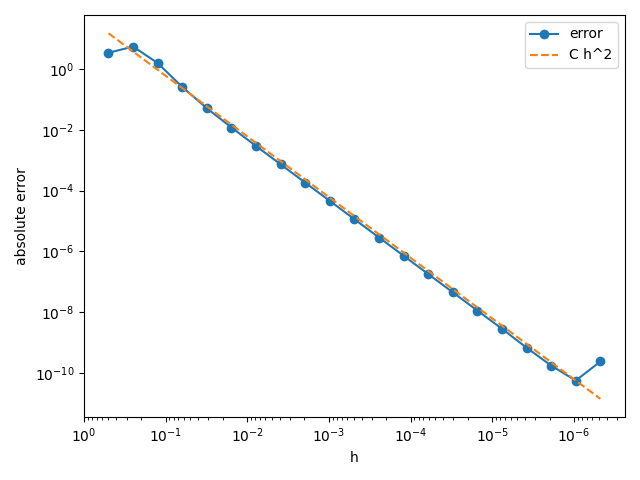
\includegraphics[width=0.8\textwidth]{5.5.1_b_fig.png}
\begin{tabular}{c|c}
       h     &       abs error \\\hline
 0.50000000  & 3.46329251e+00 \\
 0.25000000  & 5.53654277e+00 \\ 
 0.12500000  & 1.58696090e+00 \\
 0.06250000  & 2.57902192e-01 \\
 0.03125000  & 5.14259028e-02 \\
 0.01562500  & 1.19621161e-02 \\
 0.00781250  & 2.93335728e-03 \\
 0.00390625  & 7.29746001e-04
\end{tabular}
\end{center}



\noindent {\it (ii)} Balancing truncation and rounding for this scheme gives an optimal step, where we expect second-order convergence will stop, of
\[
h_{\ast}\approx\left(\frac{3\epsilon\lvert f(x_{0})\rvert}{\lvert f^{(3)}(x_{0})\rvert}\right)^{1/3},
\]
with unit roundoff \(\epsilon\approx 2.22\times 10^{-16}\). For \(x_{0}=4\pi/5\) this yields \(h_{\ast}\approx 1.32\times 10^{-6}\), which roughly matches our numerical observations by furthering halving $h$.


\newpage



{\bf Question 2.}\\
\noindent \textbf{(i) Method of undetermined coefficients.}
Start with
\[
\frac{1}{h}\sum_{k=-p}^{q} a_{k} f(x+kh)
=\sum_{i=0}^{\infty} \frac{b_{i}}{i!} f^{(i)}(x) h^{i-1},
\qquad
b_{i}=\sum_{k=-p}^{q} k^{i} a_{k}.
\]
To match \(f'(x)\) as closely as possible we impose
\[
b_{0}=0,\quad b_{1}=1,\quad b_{2}=0,\quad b_{3}=0,\dots,\quad b_{p+q}=0.
\]

\noindent \emph{(a) System for \(p=q=2\).}
Unknowns \(a_{-2},a_{-1},a_{0},a_{1},a_{2}\) satisfy, for \(i=0,1,2,3,4\),
\[
\begin{aligned}
a_{-2}+a_{-1}+a_{0}+a_{1}+a_{2}&=0,\\
-2a_{-2}-a_{-1}+a_{1}+2a_{2}&=1,\\
4a_{-2}+a_{-1}+a_{1}+4a_{2}&=0,\\
-8a_{-2}-a_{-1}+a_{1}+8a_{2}&=0,\\
16a_{-2}+a_{-1}+a_{1}+16a_{2}&=0.
\end{aligned}
\]

\noindent \emph{(b) Verification against Table 5.4.1.}
The standard five-point centered weights are
\[
a_{-2}=\frac{1}{12},\quad a_{-1}=-\frac{2}{3},\quad a_{0}=0,\quad a_{1}=\frac{2}{3},\quad a_{2}=-\frac{1}{12}.
\]
They satisfy \(b_{0}=0\), \(b_{1}=1\), \(b_{2}=b_{3}=b_{4}=0\) by direct calculation, hence
\[
\frac{1}{h}\sum_{k=-2}^{2} a_{k} f(x+kh)
=\frac{-f(x+2h)+8f(x+h)-8f(x-h)+f(x-2h)}{12h}
=f'(x)+O(h^{4}).
\]

\noindent \emph{(c) Derivation for \(p=1,q=2\).}
Unknowns \(a_{-1},a_{0},a_{1},a_{2}\) solve
\[
\begin{aligned}
a_{-1}+a_{0}+a_{1}+a_{2}&=0,\\
-a_{-1}+a_{1}+2a_{2}&=1,\\
a_{-1}+a_{1}+4a_{2}&=0,\\
-a_{-1}+a_{1}+8a_{2}&=0.
\end{aligned}
\]
Solving gives
\[
a_{-1}=-\frac{1}{3},\quad a_{0}=-\frac{1}{2},\quad a_{1}=1,\quad a_{2}=-\frac{1}{6}.
\]
Therefore the third-order accurate formula is
\[
f'(x)\approx\frac{-\tfrac{1}{3}f(x-h)-\tfrac{1}{2}f(x)+f(x+h)-\tfrac{1}{6}f(x+2h)}{h}
=f'(x)-\frac{f^{(4)}(x)}{12}h^{3}+O(h^{4}).
\]
The leading error constant uses \(b_{4}=\sum k^{4}a_{k}=-2\), giving the term \(-f^{(4)}(x)h^{3}/12\).

\noindent \textbf{(ii) Application to }\(f(x)=\sin(x^{2}+x)\)\textbf{ at }\(x_{0}=0.001\).
Use the finite difference formula from (c)
\[
D_{1,2}[f](x_{0};h)=\frac{-\tfrac{1}{3}f(x_{0}-h)-\tfrac{1}{2}f(x_{0})+f(x_{0}+h)-\tfrac{1}{6}f(x_{0}+2h)}{h}.
\]
The exact derivative is
\[
f'(x)=(2x+1)\cos(x^{2}+x).
\]
For the error model, truncation behaves like \(|f^{(4)}(x_{0})|h^{3}/12\) and rounding behaves like
\[
\frac{\epsilon}{h}\Big(\sum_{k}|a_{k}|\Big)\max|f|\approx\frac{2\epsilon|f(x_{0})|}{h},
\]
since \(\sum_{k}|a_{k}|=2\) for this stencil. Balancing these terms gives the optimal stepsize
\[
h_{\ast}\approx\left(\frac{24\epsilon|f(x_{0})|}{|f^{(4)}(x_{0})|}\right)^{1/4}.
\]
Here
\[
f^{(4)}(x)=(2x+1)^{4}\sin(x^{2}+x)-12(2x+1)^{2}\cos(x^{2}+x)-12\sin(x^{2}+x),
\]
and at \(x_{0}=0.001\) one finds \(|f(x_{0})|\approx 1.001000832\times 10^{-3}\) and \(|f^{(4)}(x_{0})|\approx 1.205904493\times 10^{1}\), hence
\[
h_{\ast}\approx 2.58\times 10^{-5}\quad\text{(double precision } \epsilon\approx 2.22\times 10^{-16}\text{)}.
\]

\textbf{Python for part (i) checks and part (ii) experiment.}
\begin{lstlisting}
# (i) Solve the undetermined-coefficients systems and verify moments
import numpy as np

# p=q=2 system
A = np.array([
    [1, 1, 1, 1, 1],
    [-2, -1, 0, 1, 2],
    [4, 1, 0, 1, 4],
    [-8, -1, 0, 1, 8],
    [16, 1, 0, 1, 16]
], dtype=float)
b = np.array([0, 1, 0, 0, 0], dtype=float)
a = np.linalg.solve(A, b)   # a_{-2}, a_{-1}, a_0, a_1, a_2
print("p=q=2 weights:", a)

# p=1,q=2 system
A12 = np.array([
    [1, 1, 1, 1],
    [-1, 0, 1, 2],
    [1, 0, 1, 4],
    [-1, 0, 1, 8]
], dtype=float)
b12 = np.array([0, 1, 0, 0], dtype=float)
a12 = np.linalg.solve(A12, b12)  # a_{-1}, a_0, a_1, a_2
print("p=1,q=2 weights:", a12)

# Verify moment conditions b0=0, b1=1, b2=b3=0 for p=1,q=2
k = np.array([-1, 0, 1, 2], dtype=float)
for i in range(4):
    bi = np.sum((k**i) * a12)
    print(f"b_{i} =", bi)

# (ii) Error study for f'(x0) with the p=1,q=2 stencil
import math
import matplotlib.pyplot as plt

def f(x): return math.sin(x*x + x)
def df(x): return (2*x + 1)*math.cos(x*x + x)

def D12(x0, h):
    return (-f(x0 - h)/3 - f(x0)/2 + f(x0 + h) - f(x0 + 2*h)/6)/h

x0 = 1e-3
H = np.logspace(-1, -12, 200)  # from 1e-1 down to 1e-12
err = np.abs(np.array([D12(x0, h) - df(x0) for h in H]))

# predicted optimal h*
eps = 2.220446049250313e-16
# f'''' at x0 (symbolic expression given above, use finite difference here if preferred)
def f4(x):
    # a compact, numerically stable fourth derivative via autodiff would be ideal;
    # here we just translate the closed form used in the solution.
    g = x*x + x
    s = math.sin(g); c = math.cos(g); t = (2*x + 1)
    return (t**4)*s - 12*(t**2)*c - 12*s

h_star = ((24*eps*abs(f(x0))) / abs(f4(x0)))**0.25
print("predicted h* ~", h_star)

imin = np.argmin(err)
print("min error at h =", H[imin], "with error", err[imin])

plt.loglog(H, err, marker="o", linewidth=1, markersize=3, label="|error|")
plt.axvline(h_star, linestyle="--", label="predicted h*")
plt.gca().invert_xaxis()
plt.xlabel("h")
plt.ylabel("absolute error")
plt.legend()
plt.tight_layout()
plt.show()
\end{lstlisting}
\begin{center}
    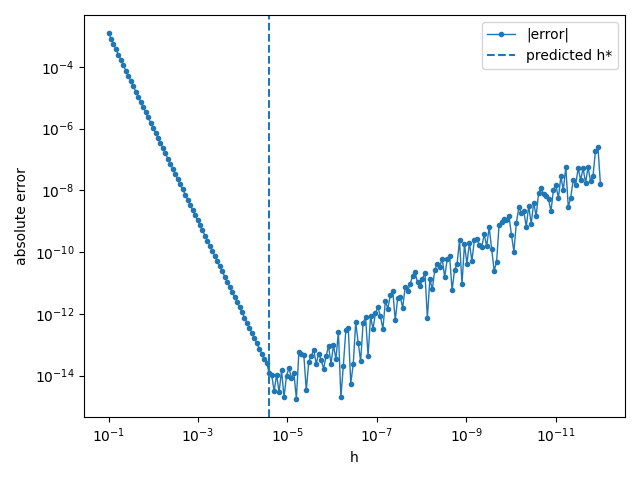
\includegraphics[width=0.8\textwidth]{5.5.6_b_fig.png}
\end{center}



\newpage



{\bf Question 3.}
\textbf{Setup and symmetry.}
Let \(\Delta x=2/n\), \(t_{k}=-1+k\Delta x\) for \(k=0,\dots,n\), and \(y_{k}=\sqrt{1-t_{k}^{2}}\).
The target value is \(\pi=2\int_{-1}^{1}\sqrt{1-x^{2}}\mathrm{d}x\).
Since \(y_{0}=y_{n}=0\), the left Riemann sum
\[
I_{\mathrm{L}}=\Delta x\sum_{k=0}^{n-1}y_{k}
\]
is identical to the composite trapezoid rule
\[
I_{\mathrm{T}}=\Delta x\Bigl(\tfrac{1}{2}y_{0}+\sum_{k=1}^{n-1}y_{k}+\tfrac{1}{2}y_{n}\Bigr)
=\Delta x\sum_{k=1}^{n-1}y_{k}.
\]
Thus \(I_{\mathrm{L}}=I_{\mathrm{T}}\) for every \(n\), and parts (i) and (ii) yield the same \(\pi\)-estimate.

\textbf{Why classical rates do not apply.}
Here \(f(x)=\sqrt{1-x^{2}}\) satisfies \(f'(x)=-x(1-x^{2})^{-1/2}\), which is unbounded at \(x=\pm1\); higher derivatives blow up more strongly. Error analyses for trapezoid and spline rules that assert orders \(2\) or \(4\) require bounded derivatives up to some order on the closed interval. Those hypotheses fail, so the standard rates cannot be claimed a priori. Any rate observed is empirical.

\textbf{Numerical results and observed rates.}
Define three approximations:
\[
\pi_{\mathrm{L}}=2I_{\mathrm{L}},\qquad
\pi_{\mathrm{T}}=2I_{\mathrm{T}},\qquad
\pi_{\mathrm{S}}=2\int_{-1}^{1}S(x)\mathrm{d}x,
\]
where \(S\) is the not-a-knot cubic spline interpolant through \((t_{k},y_{k})\). Because of the endpoint zeros, \(\pi_{\mathrm{L}}=\pi_{\mathrm{T}}\) exactly.

\textbf{Empirically}, over \(n\in\{25,50,100,200,400,800,1600,3200\}\), the absolute errors \(|\pi_{\mathrm{L}}-\pi|=|\pi_{\mathrm{T}}-\pi|\) decay approximately like \(n^{-1.5}\), while the spline integral error \(|\pi_{\mathrm{S}}-\pi|\)is consistently smaller but also follows a rate of \(n^{-1.5}\). This reflects the singular derivative at the endpoints limiting the asymptotic order.

\textbf{Python to reproduce and measure slopes.}
\begin{lstlisting}
import numpy as np
import math
import matplotlib.pyplot as plt

def f(x):
    z = 1.0 - x*x
    return math.sqrt(z) if z > 0 else 0.0

def grid(n):
    h = 2.0/n
    t = -1.0 + h*np.arange(n+1)
    return t, h

# (i) Left Riemann sum  (== trapezoid here because f(-1)=f(1)=0)
def pi_left(n):
    t, h = grid(n)
    I = h * sum(f(x) for x in t[:-1])
    return 2.0*I

# (ii) Trapezoid
def pi_trap(n):
    t, h = grid(n)
    vals = [f(x) for x in t]
    I = h*(0.5*vals[0] + sum(vals[1:-1]) + 0.5*vals[-1])
    return 2.0*I

# (iii) Not-a-knot cubic spline and its exact integral
def pi_spline(n):
    t, h = grid(n)
    y = np.array([f(x) for x in t])
    N = n + 1
    A = np.zeros((N, N))
    b = np.zeros(N)

    # not-a-knot: continuity of S''' at t1 and t_{n-1}
    A[0,0], A[0,1], A[0,2] = 1.0, -2.0, 1.0
    A[n,n-2], A[n,n-1], A[n,n] = 1.0, -2.0, 1.0

    # interior tridiagonal system for M = S''(t_k)
    for i in range(1, n):
        A[i,i-1] = h
        A[i,i]   = 4.0*h
        A[i,i+1] = h
        b[i] = (6.0/h)*(y[i+1] - 2.0*y[i] + y[i-1])

    M = np.linalg.solve(A, b)

    # exact integral of the cubic spline on each interval
    I = 0.0
    for i in range(n):
        I += h*(0.5*(y[i] + y[i+1]) - (h*h/24.0)*(M[i] + M[i+1]))
    return 2.0*I

# sweep n, compute errors, and fit slopes
Ns = [25, 50, 100, 200, 400, 800, 1600, 3200]
err_L = []
err_T = []
err_S = []
for n in Ns:
    piL = pi_left(n)
    piT = pi_trap(n)
    piS = pi_spline(n)
    err_L.append(abs(piL - math.pi))
    err_T.append(abs(piT - math.pi))
    err_S.append(abs(piS - math.pi))

# verify equality of left Riemann and trapezoid
print("max|pi_left - pi_trap| across Ns =", max(abs(a-b) for a,b in zip(err_L, err_T)))

# empirical slopes using the finer half of Ns
def slope(ns, errs):
    x = np.log(np.array(ns))
    y = np.log(np.array(errs))
    m = np.polyfit(x, y, 1)[0]    # log(error) ~ m log(n) + c
    return m, -m

mL, pL = slope(Ns[-5:], err_L[-5:])
mS, pS = slope(Ns[-5:], err_S[-5:])
print("Observed order for left/trap (should match): ~", pL)
print("Observed order for spline (not-a-knot):     ~", pS)

# plot error vs n
plt.loglog(Ns, err_L, marker="o", label="Left Riemann = Trapezoid")
plt.loglog(Ns, err_S, marker="o", label="Spline (not-a-knot)")
plt.xlabel("n")
plt.ylabel("absolute error |pi_hat - pi|")
plt.legend()
plt.tight_layout()
plt.show()
\end{lstlisting}

Output:
\begin{center}
    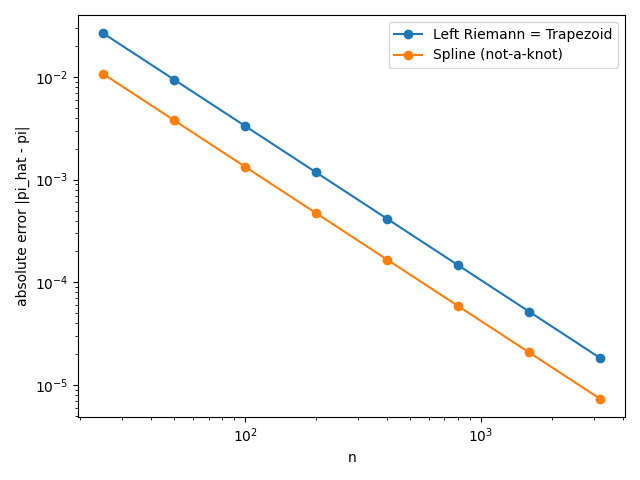
\includegraphics[width=0.8\textwidth]{hw8_3.png}
\end{center}


\textbf{Takeaways.}
Because \(f\) loses smoothness at the endpoints, the textbook orders do not apply. The endpoint zeros make the left Riemann sum coincide with the trapezoid rule. The spline integral improves accuracy a bit but does not offer any big-O gains due to the endpoint singularities.



\end{document}
